% Point d'avancement tuteur, 31 juillet 2026. Compile avec Tectonic (pdfLaTeX standard).
% Perimetre : TOUT ce qui a ete fait depuis le point du 24/07. Deux blocs :
%   (A) les quatre pistes demandees au call du 24/07 (NB, seuil P4, W=S+A, KPI) ;
%   (B) ce qui a suivi : la remarque de Caroline Hillairet et la robustesse, puis la
%       DIRECTION de la contagion cherchee dans les rapports d'enquete, qui debouche sur
%       une demande de relecture croisee.
% Regle de presentation : aucun niveau de SCR agrege n'est affiche, seulement des ecarts,
% des rapports et des structures.
\documentclass[11pt]{beamer}
\usetheme{Madrid}
\usecolortheme{seahorse}
\usepackage[utf8]{inputenc}
\usepackage[T1]{fontenc}
\usepackage[french]{babel}
\usepackage{booktabs}
\usepackage{amsmath,amssymb}
\usepackage{eurosym}
\graphicspath{{../vasicek_lab/figures/}{../cascade_qualitative/figures/}}
\setbeamertemplate{navigation symbols}{}
\setbeamertemplate{caption}{\raggedright\insertcaption\par}
\setbeamerfont{block title}{size=\small}

\title[Point d'avancement]{Mémoire SCR DORA : point d'avancement}
\subtitle{Les quatre pistes du 24/07, et ce qu'elles ont ouvert}
\author[K. Kaddouri]{Kélian Kaddouri}
\institute[ENSAE / Nexialog]{ENSAE / Nexialog Consulting}
\date[31/07/2026]{31 juillet 2026}

\begin{document}

\begin{frame}
\titlepage
\end{frame}

% =====================================================================
\begin{frame}{Depuis le dernier point}
Au call du 24/07, quatre pistes : \textbf{approfondir les KPI}, la \textbf{simulation de la loi
de comptage}, le \textbf{seuil de déclenchement de P4}, et la \textbf{décomposition symétrique
et antisymétrique} rapprochée de la martingalisation.
\medskip

Les quatre sont traitées. Chacune est un script et une figure, vérifiée numériquement. Mais
elles en ont ouvert deux autres, qui occupent la seconde moitié de ce point.
\vfill
\begin{block}{Le plan}
\textbf{(A)} Les quatre pistes demandées.\\[3pt]
\textbf{(B)} Ce qu'elles ont ouvert : la remarque de \textbf{Caroline Hillairet} sur le
quantile, qui conduit à expliciter l'incertitude et à valider le socle ; puis la
\textbf{direction de la contagion}, que je n'arrivais pas à calibrer et que je suis allé
chercher ailleurs. Sur ce dernier point, j'ai un \textbf{service à te demander}.
\end{block}
\end{frame}

% =====================================================================
\section*{A. Les quatre pistes}

\begin{frame}{Piste : la loi de comptage, simulée et réconciliée}
\begin{center}
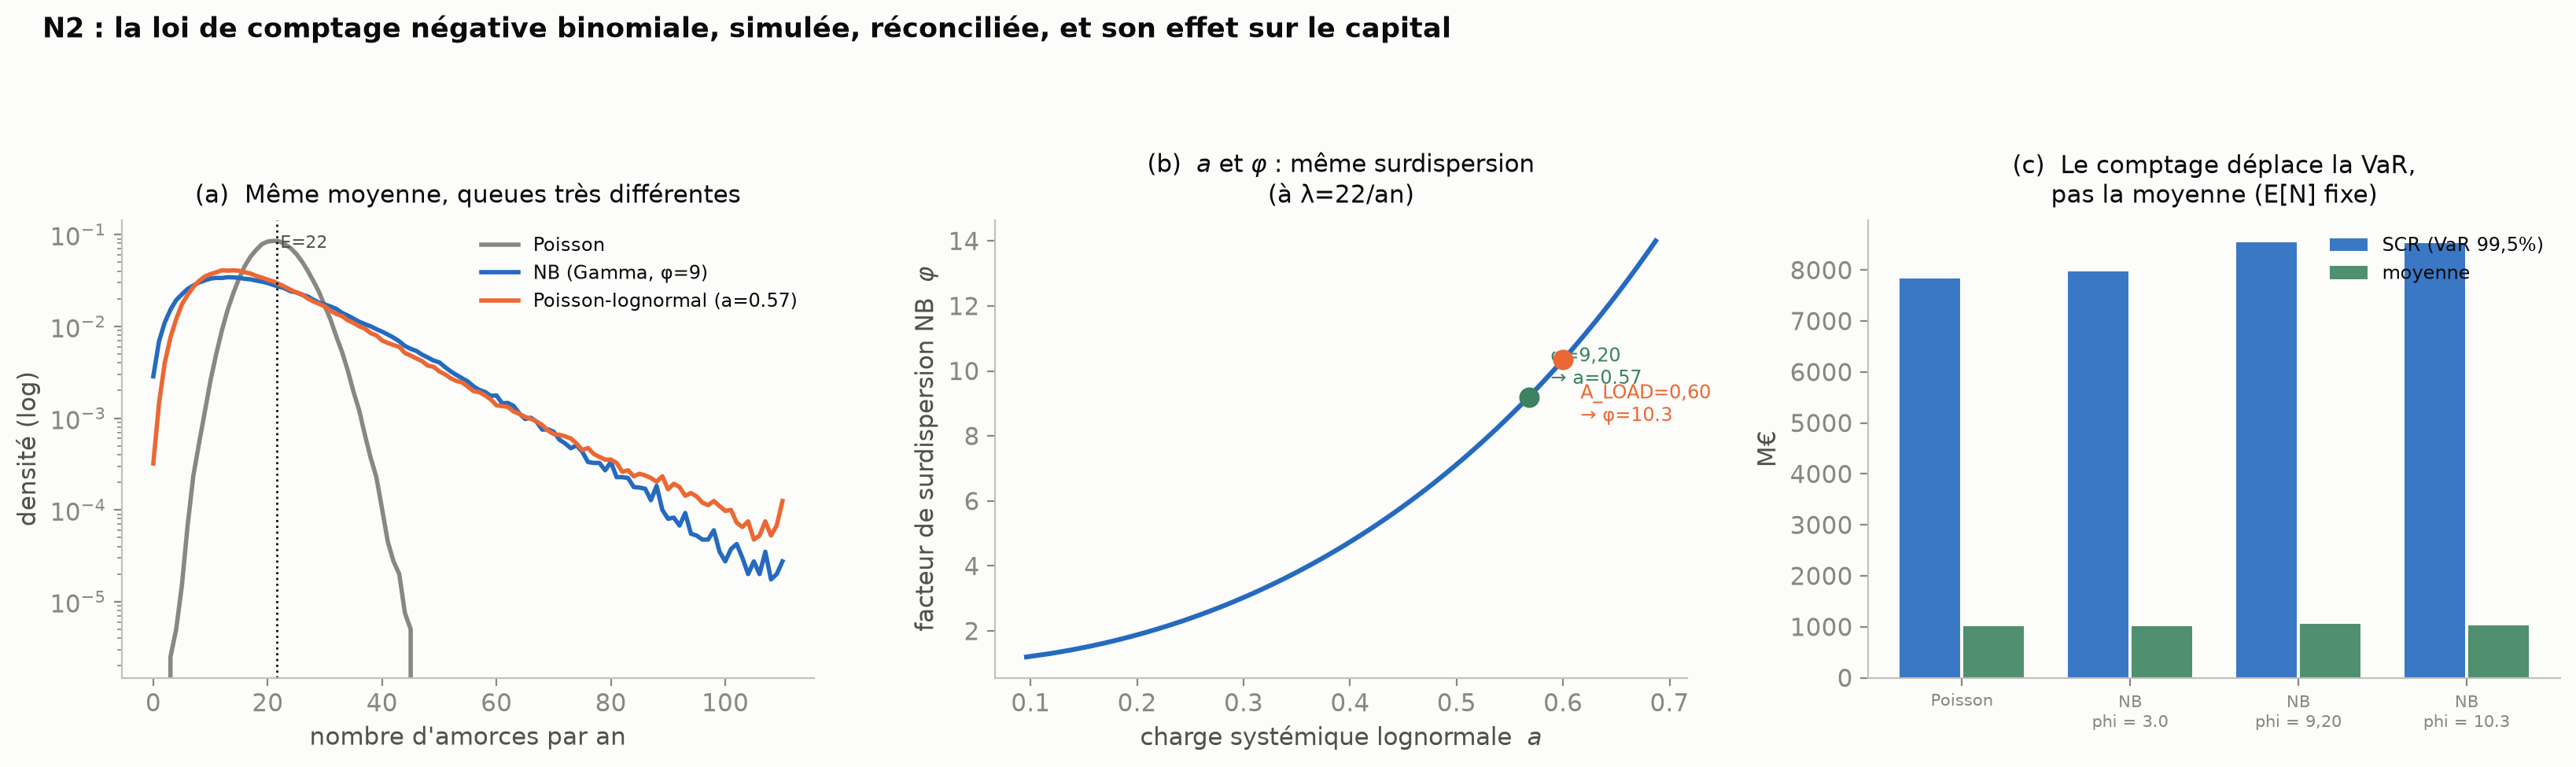
\includegraphics[width=\linewidth]{N2_simulation_nb.png}
\end{center}
\vspace{-2mm}
\small
Le modèle portait \textbf{trois} mesures de surdispersion jamais confrontées. La charge
systémique et le facteur négatif binomial sont en fait \textbf{la même} surdispersion agrégée
(elles coïncident à $5\,\%$). À variance égale, la queue dépend encore de la loi de mélange
($+11\,\%$). Et le comptage \textbf{déplace la VaR, pas la moyenne}. La série détrendée donne
une surdispersion trois fois plus faible que celle retenue : le calage actuel est
\textbf{conservateur, pas calibré}, à assumer comme tel.
\end{frame}

% =====================================================================
\begin{frame}{Piste : le seuil de déclenchement de P4}
Deux questions distinctes, et la loi normale ne convient qu'à la première.
\begin{itemize}
\item \textbf{La marge} (quand P4 bascule) : franchissement $X_4 \ge K_4$, où la loi de la
      latente n'est qu'une \textbf{normalisation}. La queue lourde du capital est dans la
      \textbf{sévérité}, pas ici : la normale y est inoffensive.
\item \textbf{La dépendance} (combien de piliers ensemble) : là, une copule gaussienne a une
      dépendance de queue \textbf{nulle} et sous-estime le basculement simultané. Elle
      contredit la copule de Gumbel retenue ailleurs dans le mémoire.
\end{itemize}
\vfill
\begin{block}{On borne l'accumulation, dans l'esprit du mémoire}
À dépendance moyenne égale, l'accumulation est encadrée du \textbf{plancher gaussien} au
\textbf{haut de Gumbel}. La marge est invariante ; seule la co-occurrence de queue bouge. Le
co-extrême (les \textbf{cinq} piliers avec P4) passe de $0{,}17$ à $0{,}39$ : c'est le scénario
MOVEit, que la queue gaussienne manque.
\end{block}
\end{frame}

% =====================================================================
\begin{frame}{Piste : $W = S + A$ comme réversibilité d'un processus}
\begin{center}
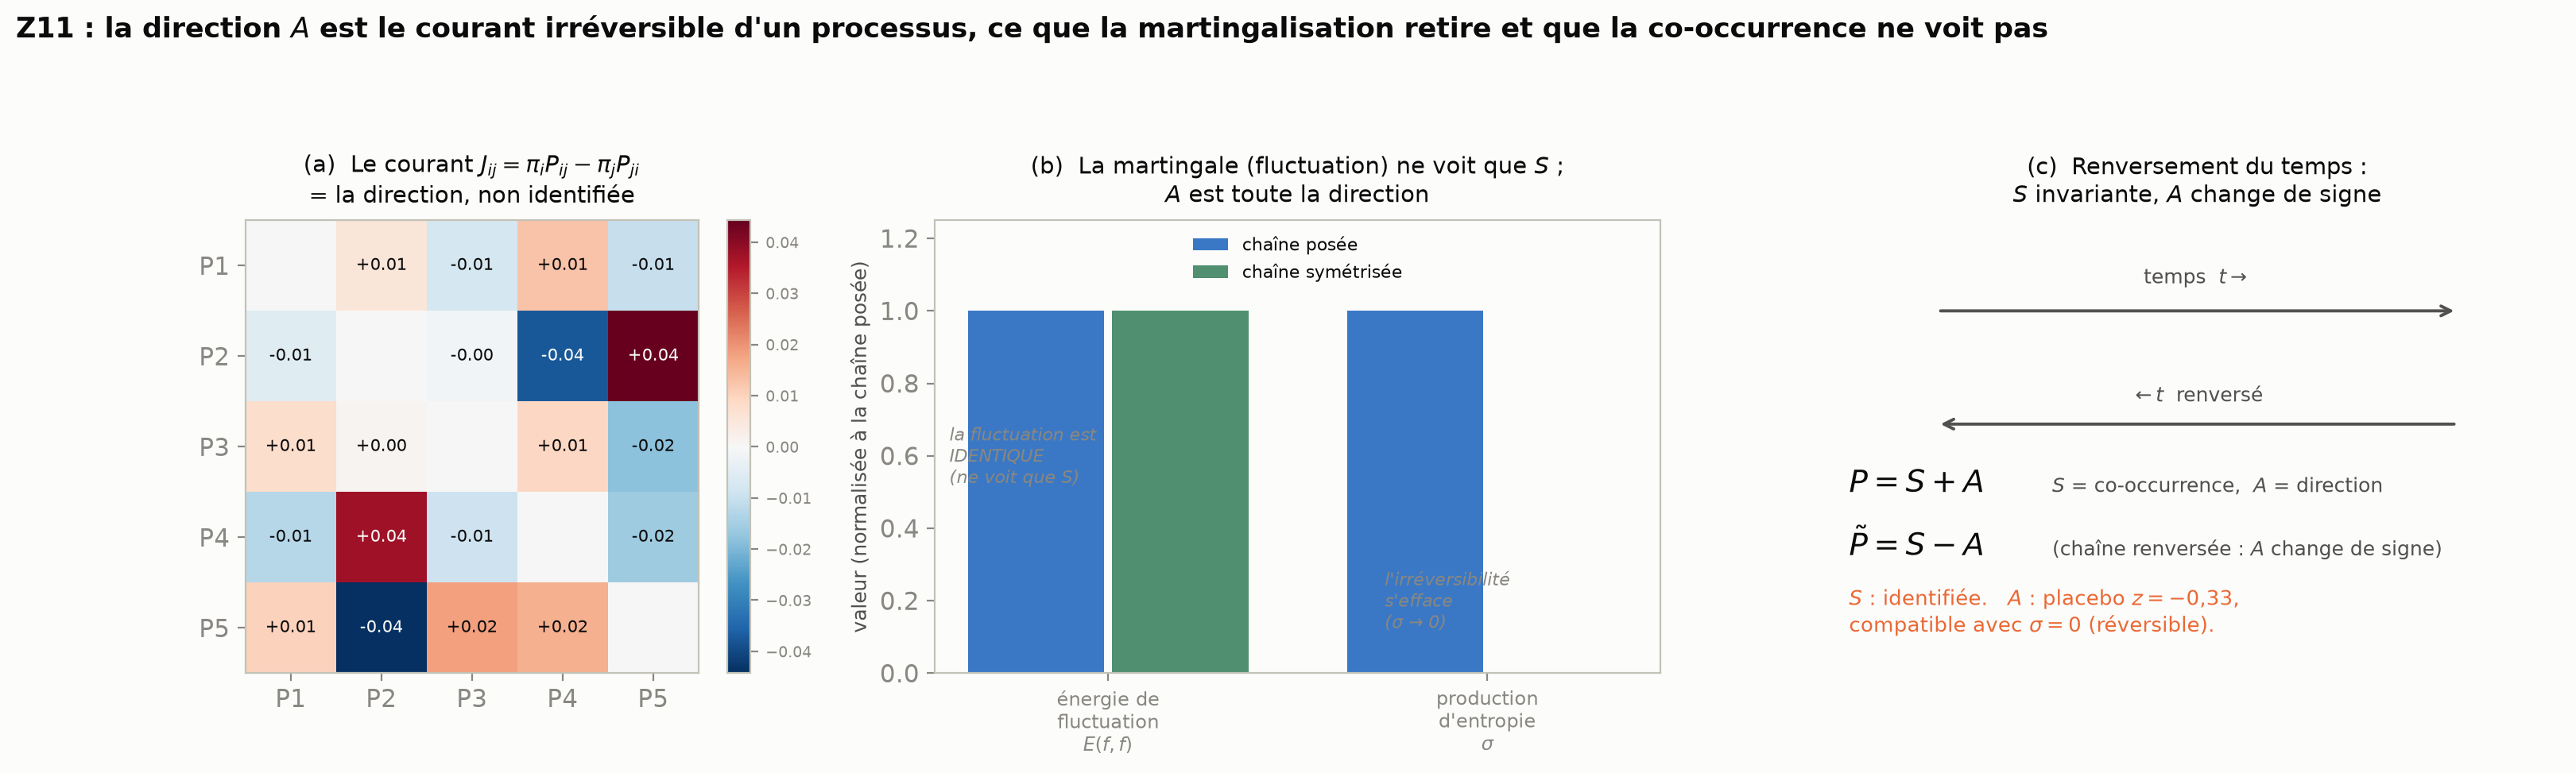
\includegraphics[width=\linewidth]{Z11_reversibilite_martingale.png}
\end{center}
\vspace{-2mm}
\small
Le parallèle avec la martingalisation est \textbf{faisable}, et il \textbf{fonde} la limite
d'identification au lieu de la constater. La direction $A$ est le \textbf{courant irréversible}
d'un processus : la fluctuation, c'est-à-dire la martingale, ne voit que $S$, et le renversement
du temps retourne $A$ mais laisse $S$ intacte. Le placebo $z=-0{,}33$ se relit alors comme une
donnée \textbf{compatible avec l'équilibre détaillé} : une statistique invariante par
renversement ne peut pas identifier un courant qui change de signe sous ce renversement.
\end{frame}

% =====================================================================
\begin{frame}{Piste : des KPI descriptifs aux KPI pilotables}
\begin{center}
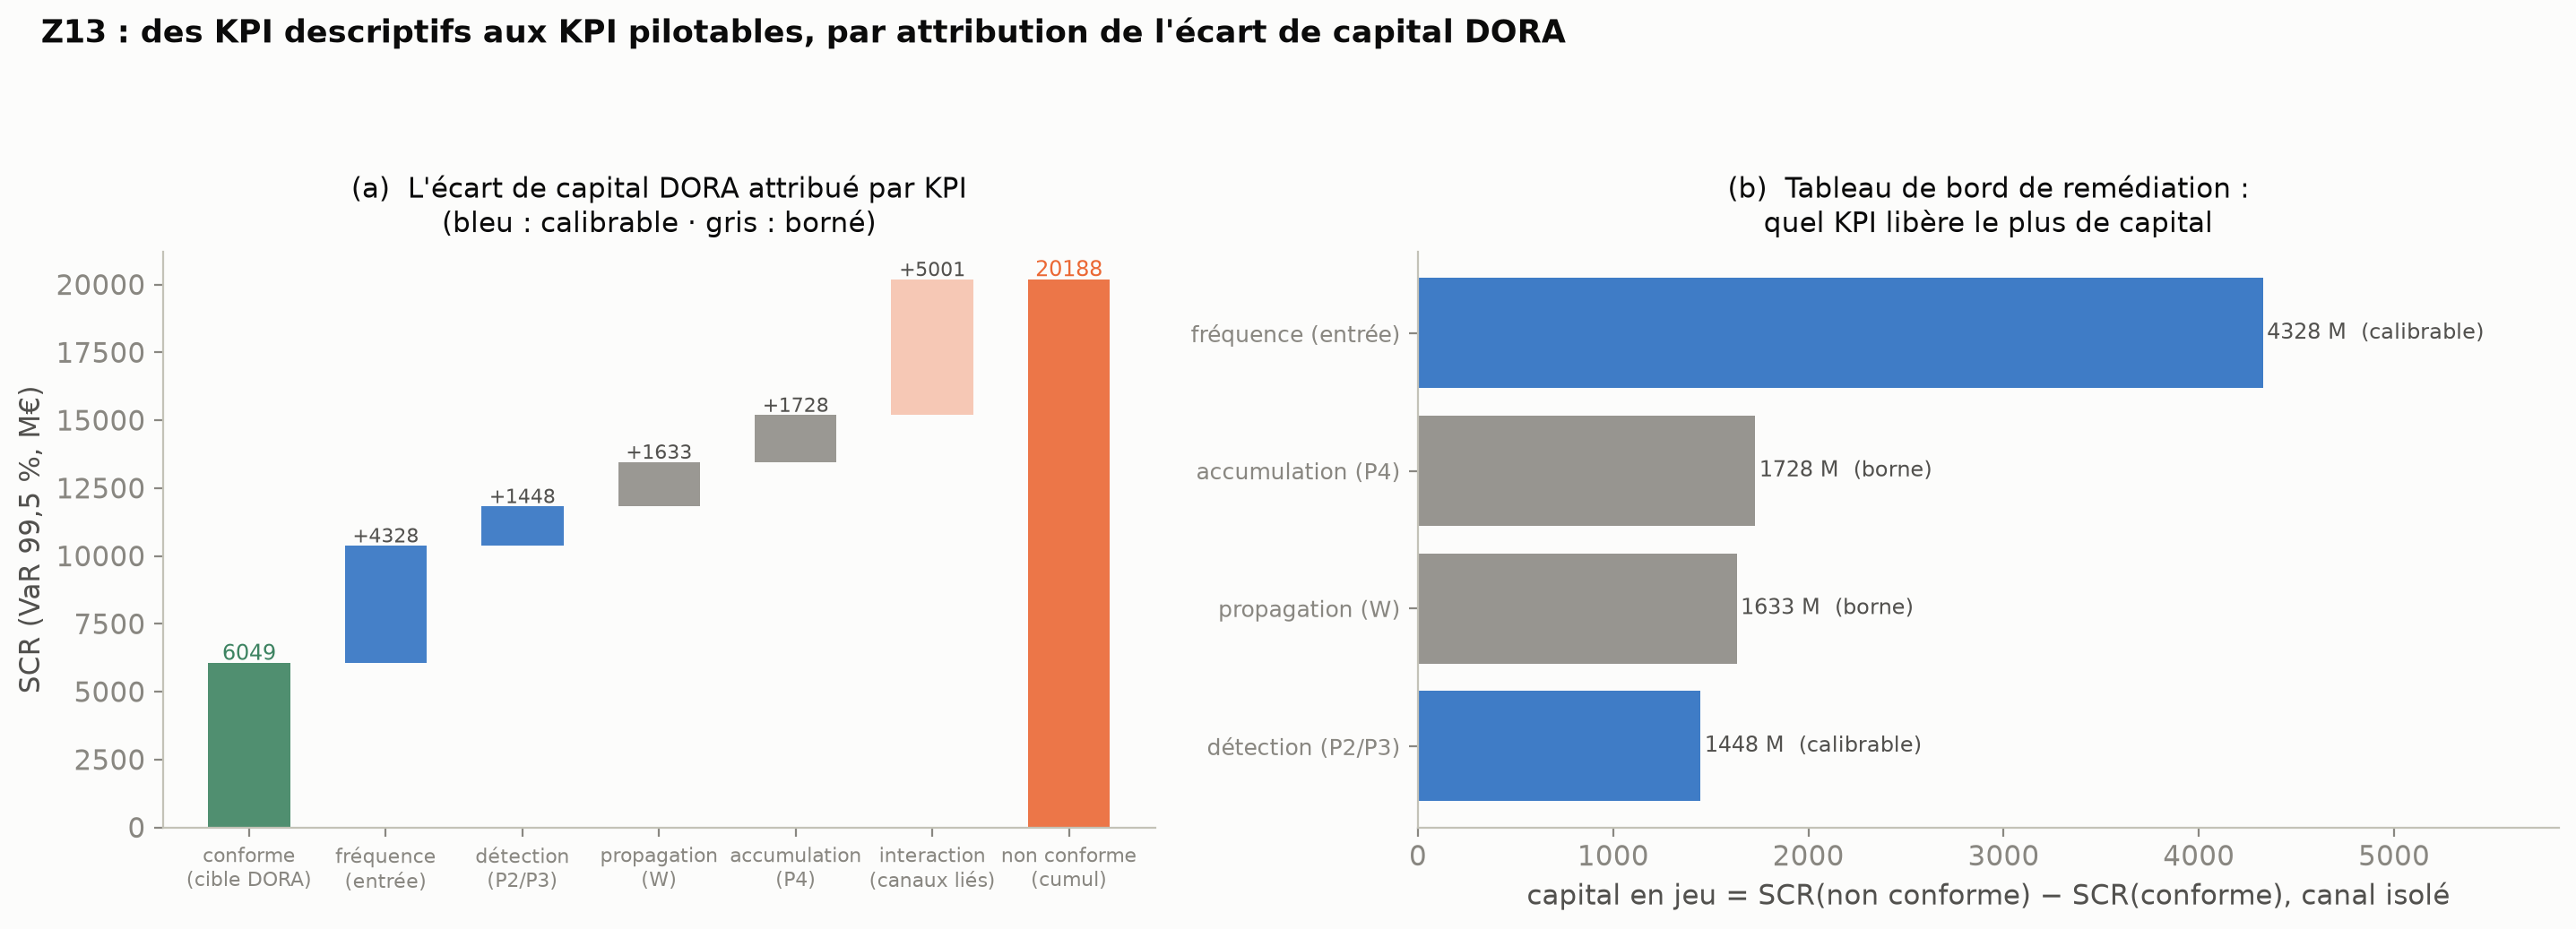
\includegraphics[width=\linewidth]{Z13_kpi_pilotables.png}
\end{center}
\vspace{-2mm}
\small
Chaque indicateur observable est rattaché à un canal du moteur, et l'on mesure le
\textbf{capital en jeu} derrière lui. L'essentiel n'est pas le montant mais sa
\textbf{concentration} : quelques leviers portent l'essentiel du capital libéré, ce qui permet
de \textbf{prioriser} la remédiation plutôt que de l'étaler. On passe du score de criticité
abstrait à un \textbf{arbitrage économique de priorisation}, opposable à une direction
financière.
\end{frame}

% =====================================================================
\section*{B. Ce que ces pistes ont ouvert}

\begin{frame}{La remarque de Caroline : un quantile d'un objet incertain}
\og{}Prendre le quantile de quelque chose d'incertain est mauvais.\fg{}
\medskip

Le SCR est une VaR $99{,}5\,\%$ : un point de la queue, lu là où les données sont les plus
rares. Sur nos données, son seul intervalle de confiance vaut déjà un \textbf{facteur 2,6}.
\vfill
\begin{block}{La réponse}
On ne peut pas abandonner la VaR, imposée par le cadre prudentiel. On \textbf{explicite} donc
l'incertitude, sur trois étages qui se cumulent : \textbf{paramètre} (bootstrap),
\textbf{identification} (bornes sur la direction), et \textbf{modèle} (le choix de la famille
elle-même). Loin d'attaquer l'approche, la remarque en est la justification.
\end{block}
\end{frame}

% =====================================================================
\begin{frame}{Les trois étages de l'incertitude}
\begin{center}
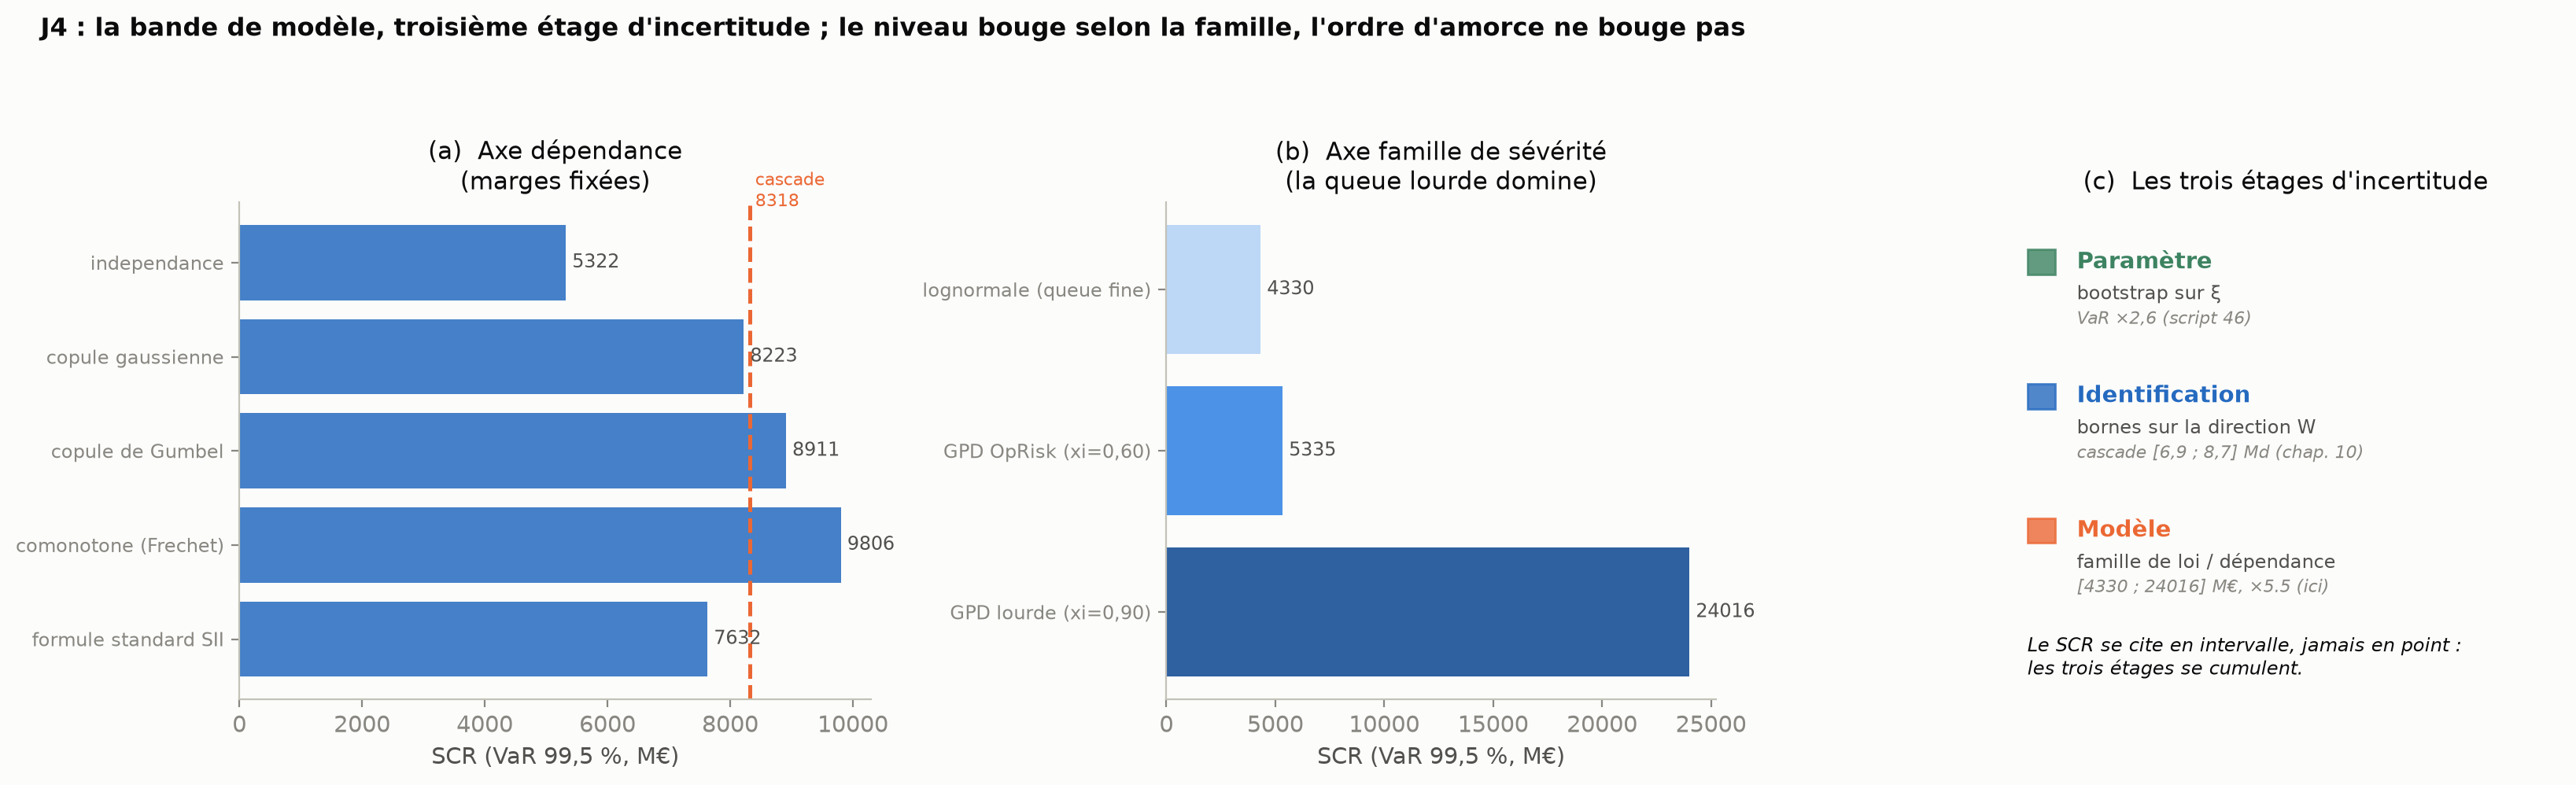
\includegraphics[width=\linewidth]{J4_bande_modele.png}
\end{center}
\vfill
\footnotesize À marges fixées, la structure de \textbf{dépendance} déplace le SCR d'un facteur
$1{,}8$, notre cascade tombant entre les copules gaussienne et de Gumbel ; la \textbf{famille de
queue}, d'un facteur $5{,}5$. \textbf{Le niveau bouge dans la bande, l'ordre des piliers ne bouge
pas} : c'est la thèse du mémoire, chiffrée sur un troisième axe.
\end{frame}

% =====================================================================
\begin{frame}{Le socle passe les tests d'adéquation}
\begin{center}
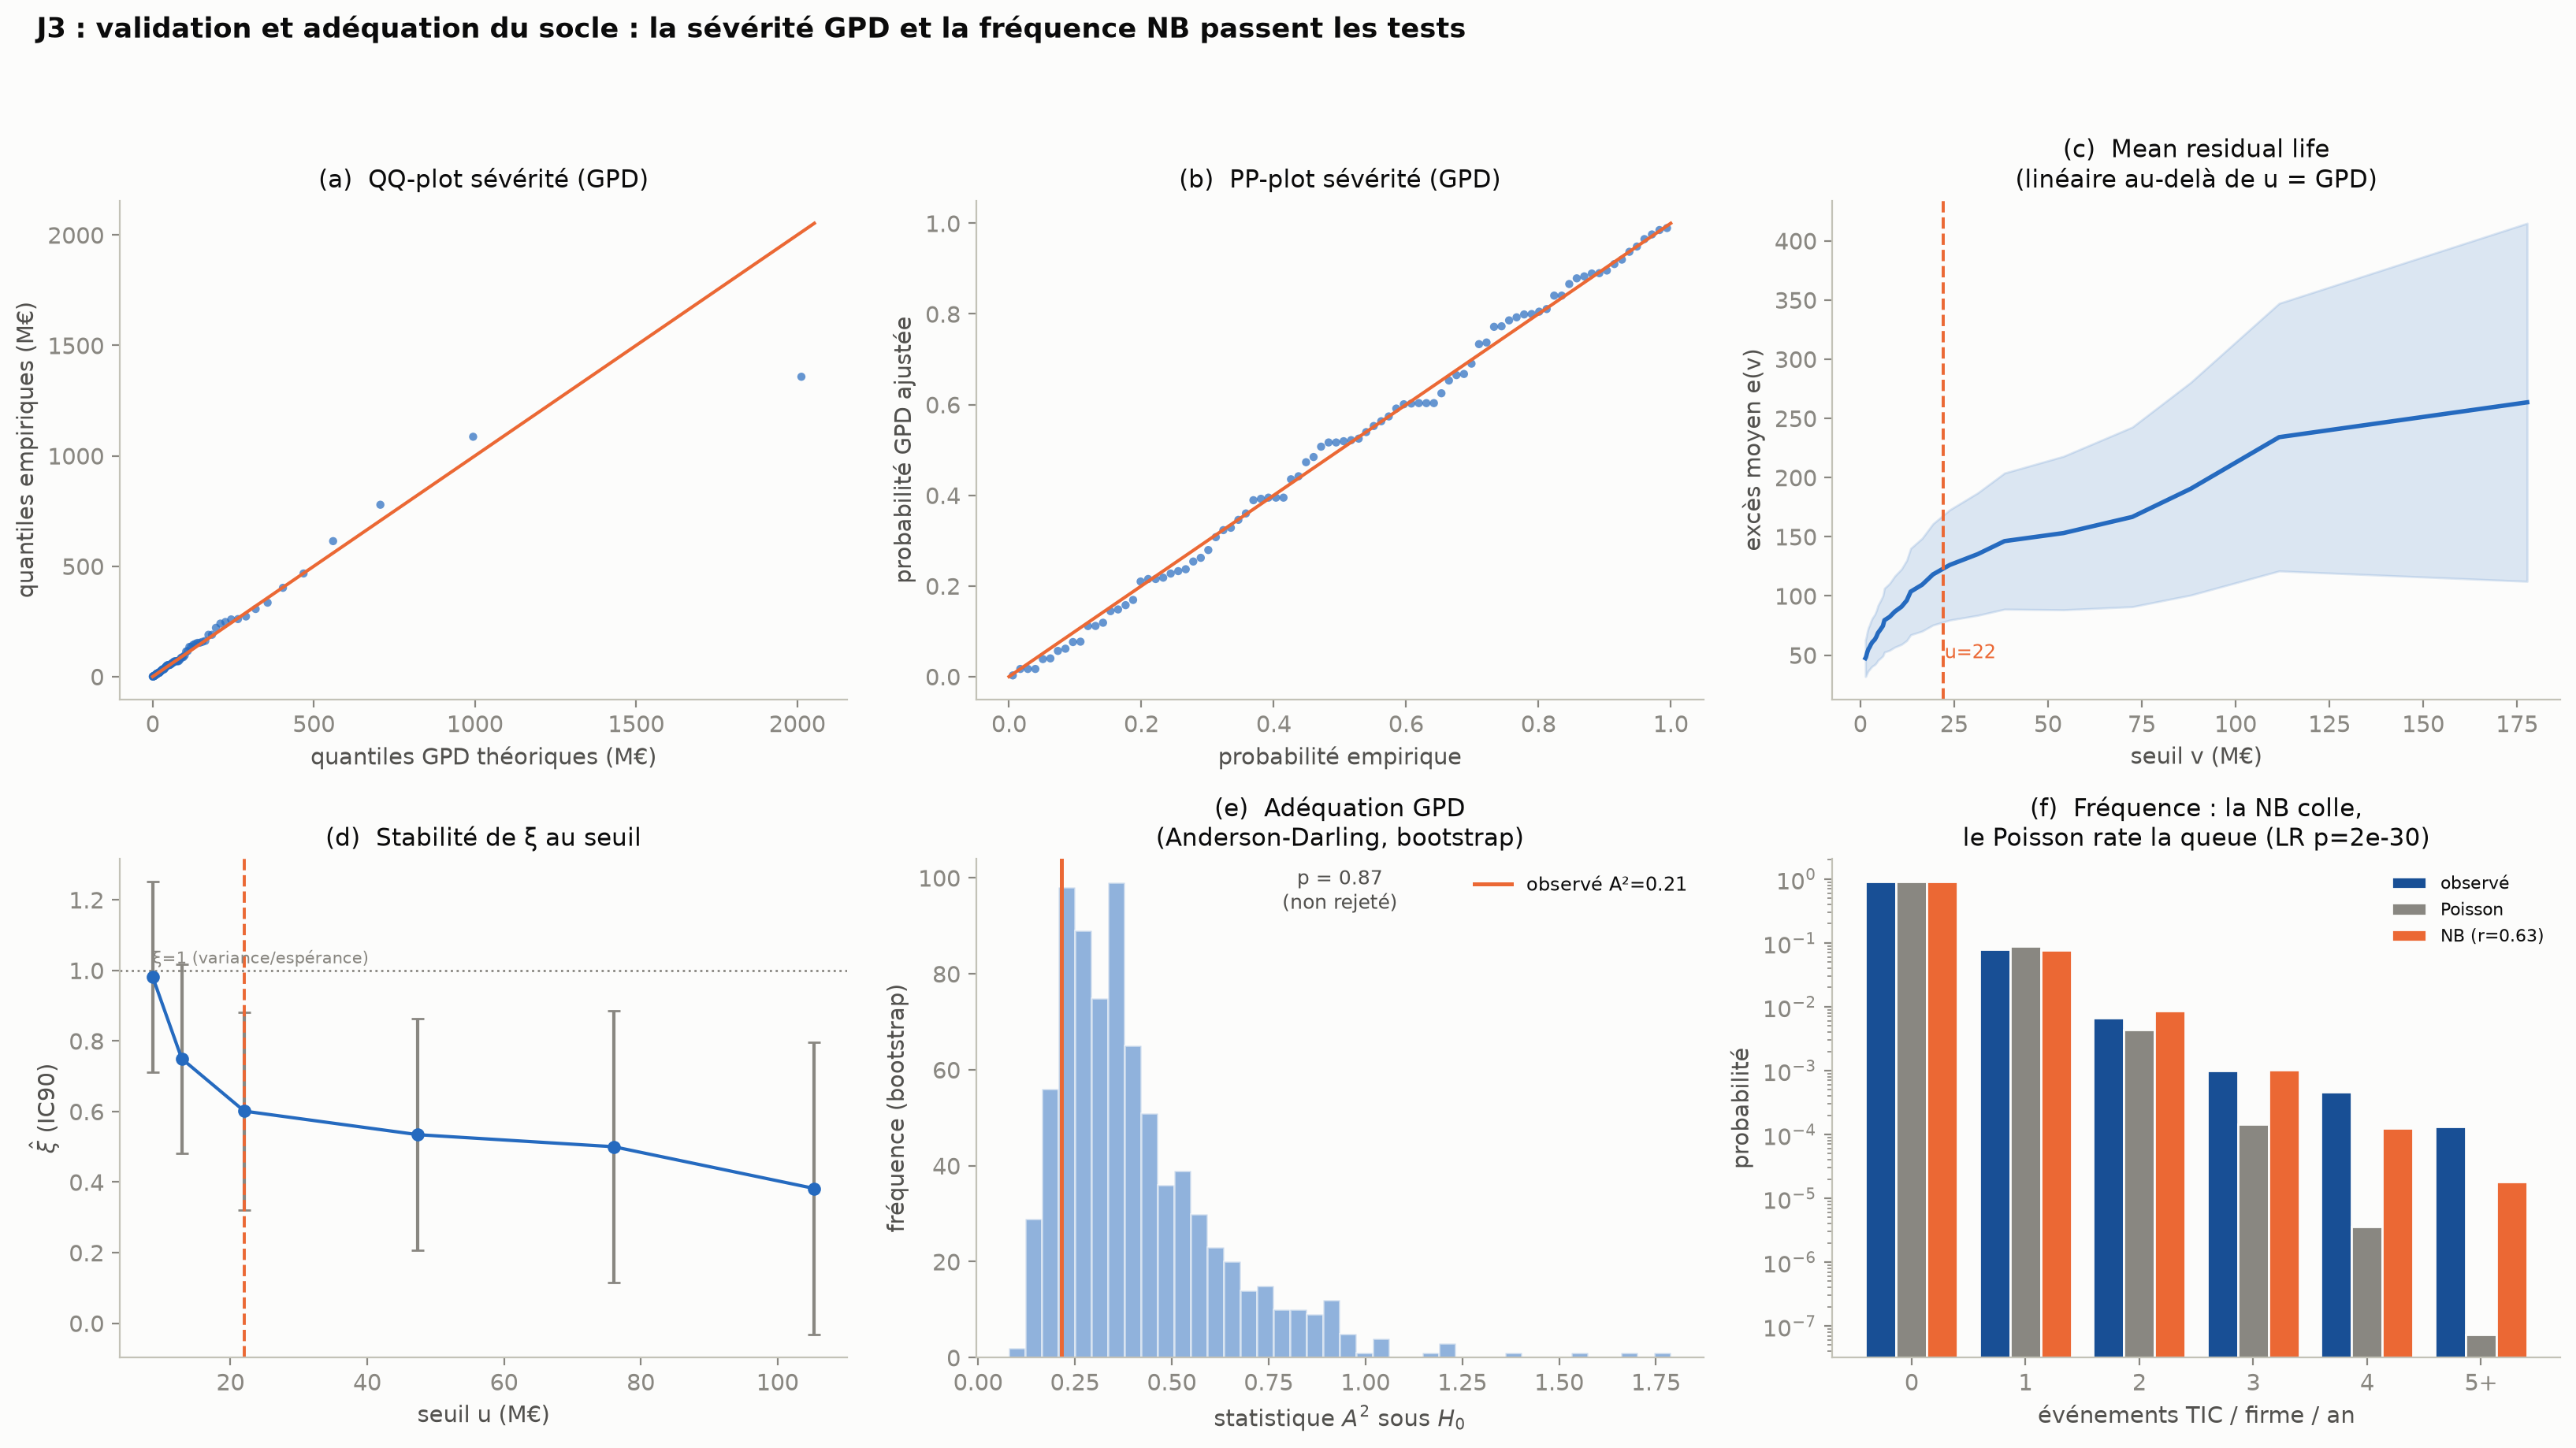
\includegraphics[width=0.80\linewidth]{J3_validation_adequation.png}
\end{center}
\vspace{-2mm}
\footnotesize\centering
\textbf{Sévérité} : tracés sur la diagonale, vie résiduelle moyenne linéaire, indice de queue
stable, tests non rejetés ($p=0{,}87$, par bootstrap paramétrique). \textbf{Fréquence} : la
négative binomiale domine le Poisson sans ambiguïté. Les \emph{formes} sont validées ; le
\emph{niveau} reste une bande.
\end{frame}

% =====================================================================
\begin{frame}{La direction, cherchée ailleurs que dans les bases}
\small
Aucune base publique ne mesure le \emph{sens} de la contagion, et le mémoire en fait un
résultat. Mais l'information existe ailleurs : après chaque grand incident, une \textbf{enquête
publique} reconstitue la séquence des défaillances. C'est la donnée qui manquait, à l'intérieur
d'un document et non d'une base.
\vfill
\begin{block}{Sept rapports dépouillés}
Microsoft Exchange, TSB, Equifax, Knight Capital, Capital One, ION, MOVEit.
\textbf{17 enchaînements} codés, protocole explicite.
\end{block}
\begin{block}{}
Le test placebo est cette fois \textbf{franchi} ($z=+3{,}9$ contre $-0{,}33$ sur les bases
agrégées), \textbf{aucun} enchaînement ne va à contre-sens, et la \textbf{gouvernance n'est
jamais une cible} quand la \textbf{gestion des incidents} est un aboutissement : la structure du
classeur, retrouvée par un chemin indépendant.
\end{block}
\end{frame}

% =====================================================================
\begin{frame}{Ce que cette information vaut, et laquelle chercher d'abord}
\begin{center}
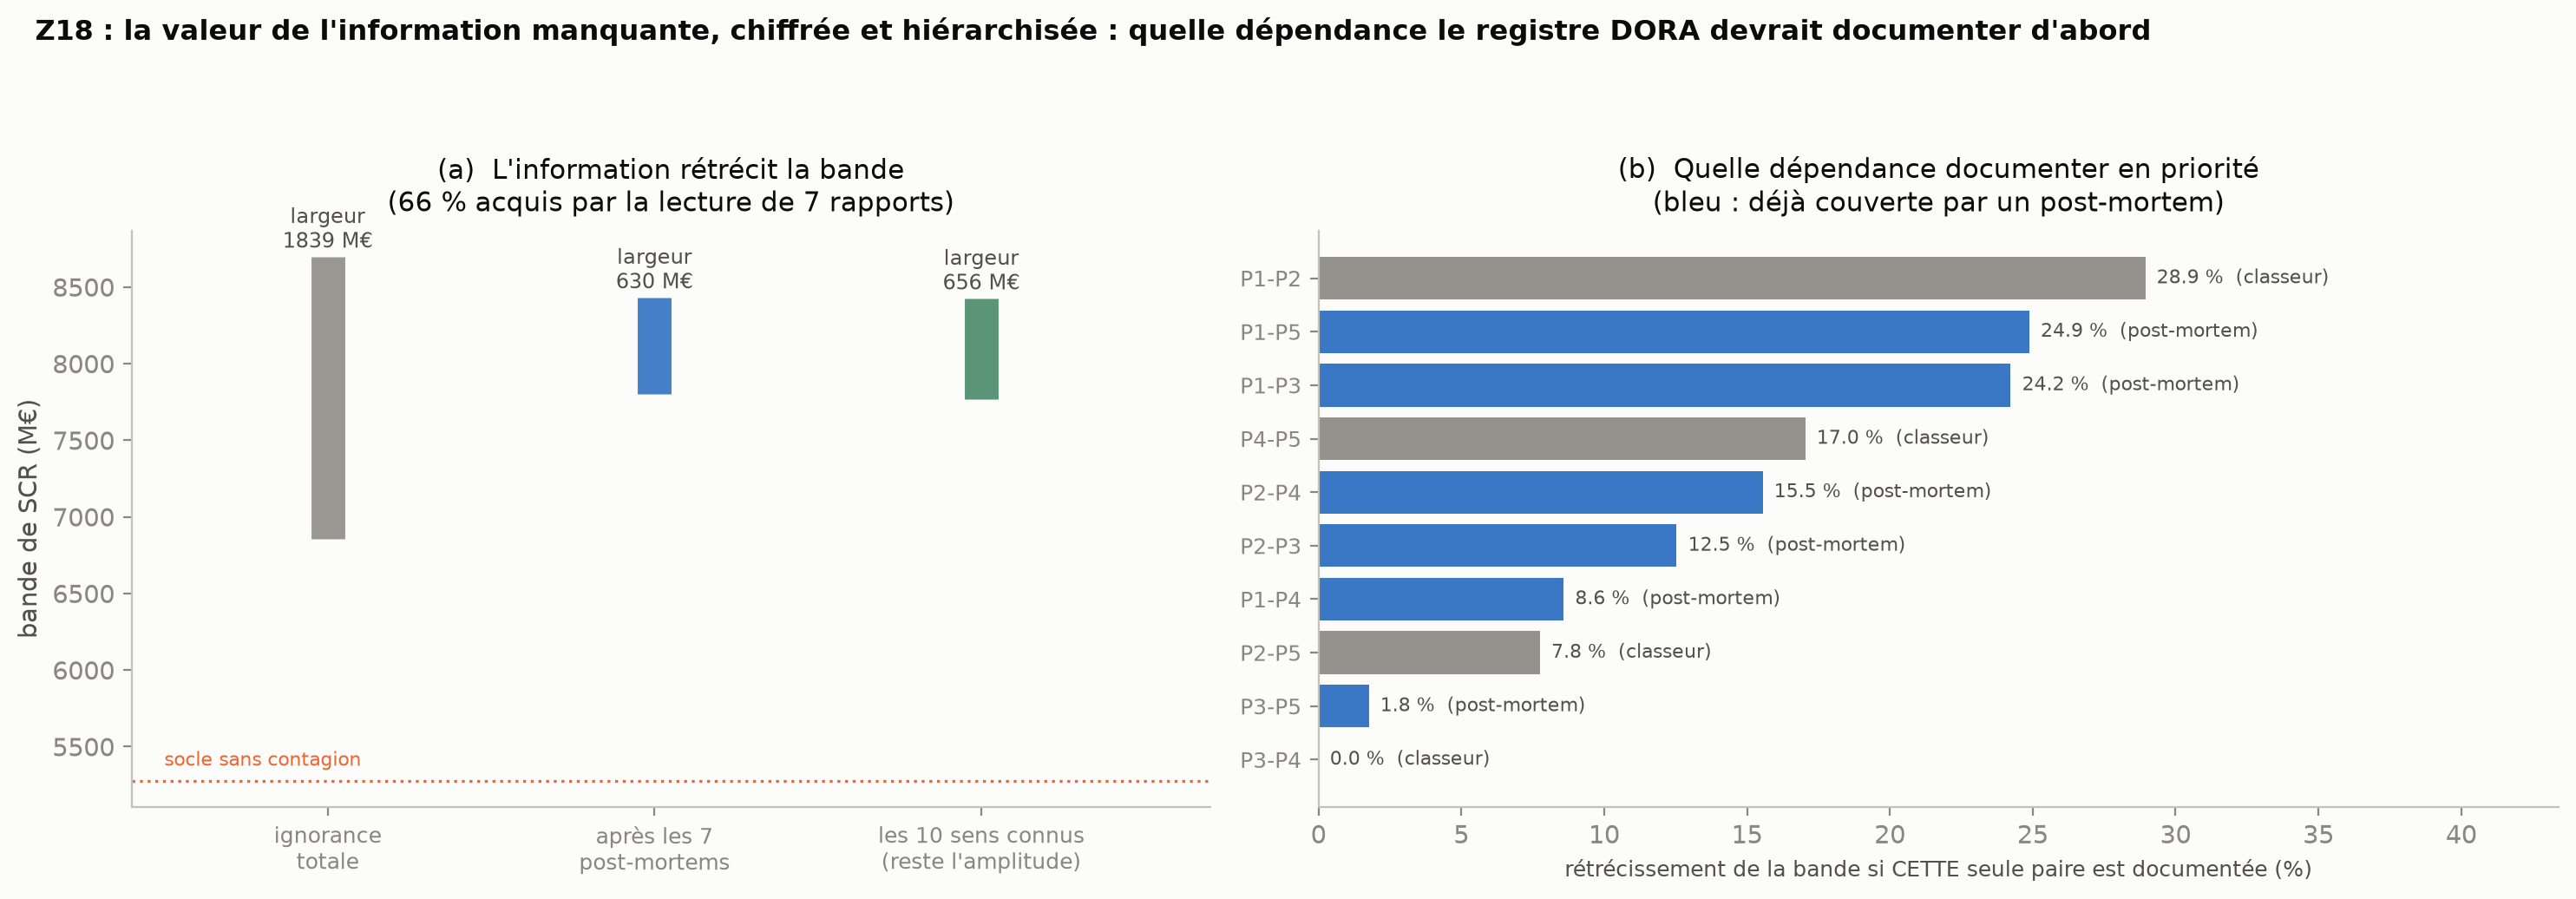
\includegraphics[width=\linewidth]{Z18_valeur_information.png}
\end{center}
\vspace{-2mm}
\small
Lire ces sept rapports a levé \textbf{66 \%} de l'ambiguïté sur la direction. Surtout, cette
valeur se \textbf{hiérarchise} : documenter une seule dépendance (gouvernance vers gestion des
incidents) en lèverait \textbf{29 \%} à elle seule, une autre n'en lèverait \emph{rien}. La
recommandation faite au régulateur cesse d'être générique. Et la dépendance la plus précieuse
est justement celle que les rapports ne couvrent pas.
\end{frame}

% =====================================================================
\begin{frame}{Ce que je ne revendique pas, et le service que je demande}
\begin{center}\small
\renewcommand{\arraystretch}{1.3}
\begin{tabular}{@{}l l l@{}}
\toprule
\textbf{Objet} & \textbf{Ce que j'ai} & \textbf{Posture} \\
\midrule
La structure d'ensemble & 17 enchaînements cohérents & \textbf{revendiquée} \\
Le sens de chaque lien & 2 paires sur 6 concluantes & \textbf{non revendiquée} \\
La force des liens & rien, et rien ne la donnera & \textbf{hors d'atteinte} \\
\bottomrule
\end{tabular}
\end{center}
\vfill
\begin{block}{La faiblesse que je préfère traiter plutôt que subir}
\small Ce dépouillement, \textbf{je l'ai fait seul}. Et une enquête cherche un responsable :
elle conclut presque toujours à un défaut de gouvernance. L'ordre trouvé pourrait refléter la
\textbf{façon d'écrire ces rapports} plutôt que le terrain.
\end{block}
\begin{block}{D'où deux demandes, courtes et sans mathématiques}
\small
\textbf{1. Codage en aveugle} (45 min), par quelqu'un \textbf{hors du projet} : donc pas toi, et
c'est précisément le point. \emph{Qui verrais-tu chez Nexialog ?}\\[2pt]
\textbf{2. Relecture de praticien} (30 min) : \emph{toi}, et \emph{Mehdi} à son retour.
\end{block}
\end{frame}

% =====================================================================
\begin{frame}{P4 au niveau sous-process, et le fil qui se referme}
\begin{columns}
\begin{column}{0.52\linewidth}
\centering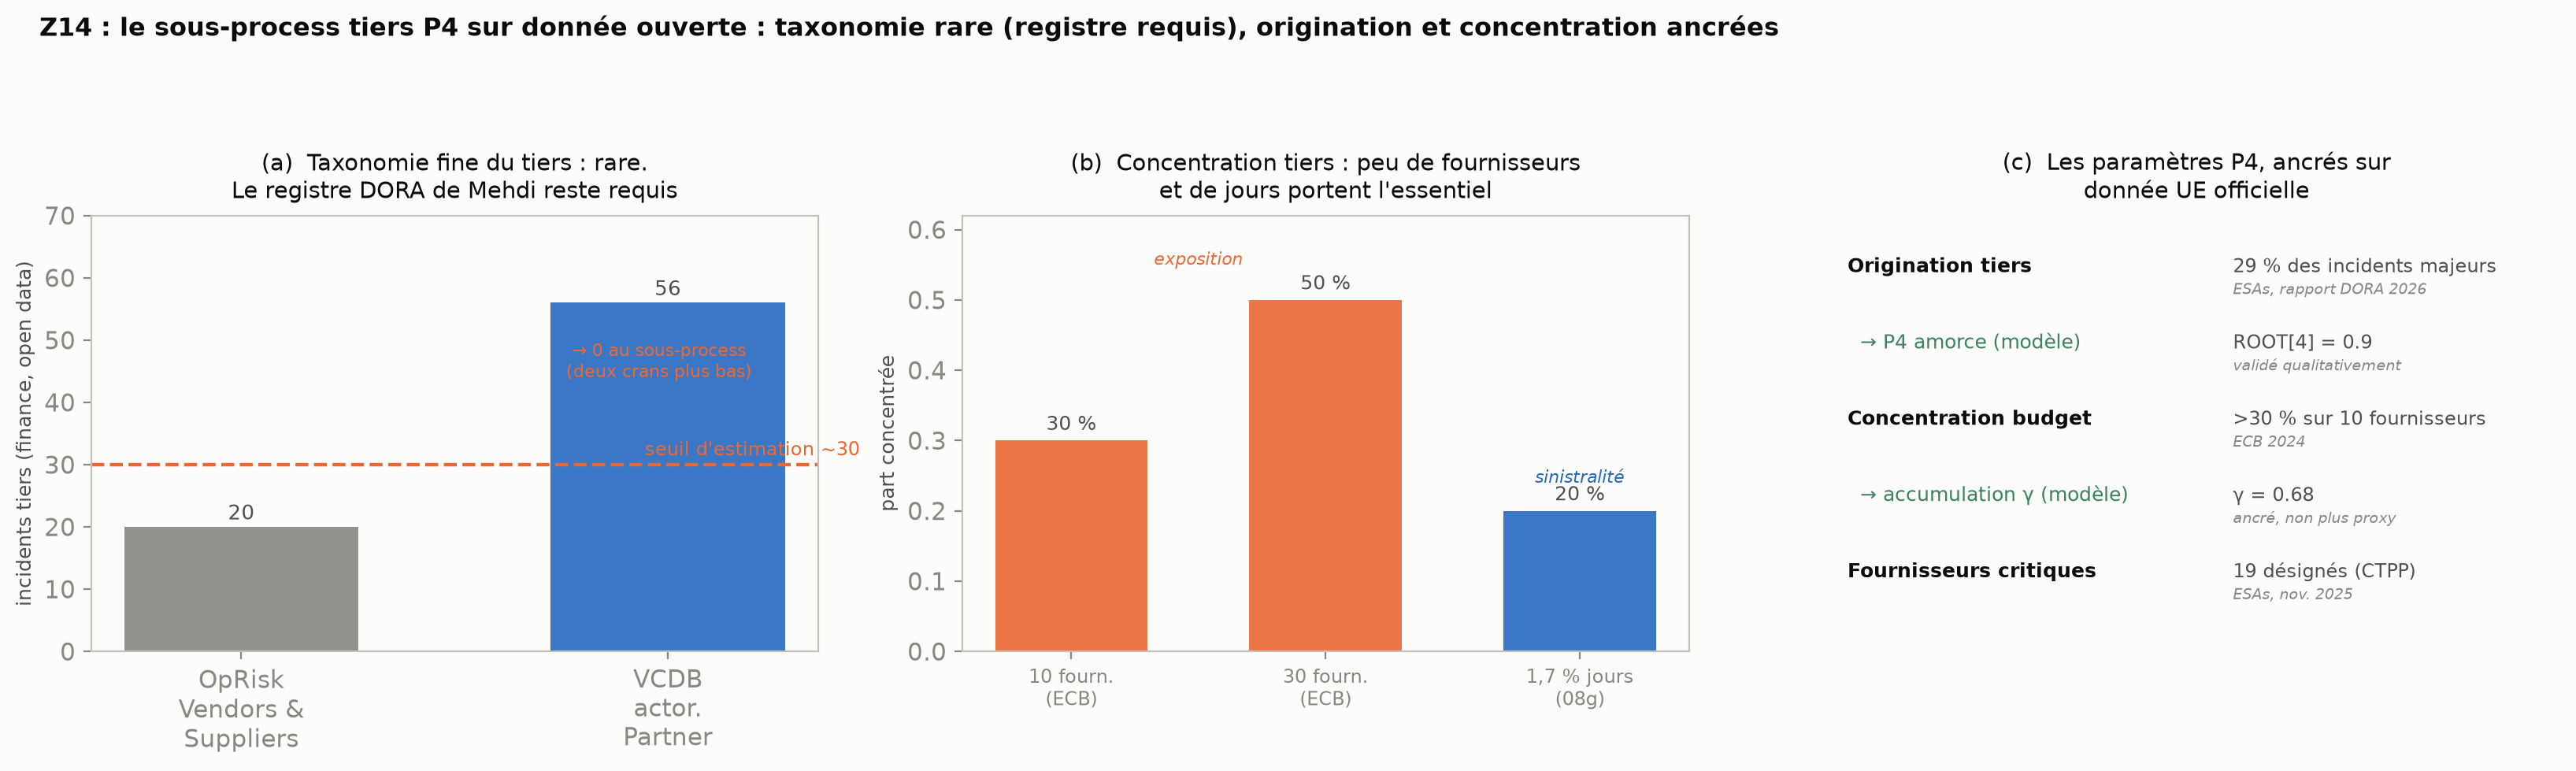
\includegraphics[width=\linewidth]{Z14_p4_sousprocess_open.png}\\[2pt]
{\scriptsize La taxonomie fine du tiers est rare : le registre reste requis. Mais
l'\textbf{origination} ($29\,\%$ des incidents majeurs d'origine tierce) et la
\textbf{concentration} sont ancrées sur donnée européenne officielle.}
\end{column}
\begin{column}{0.45\linewidth}
\centering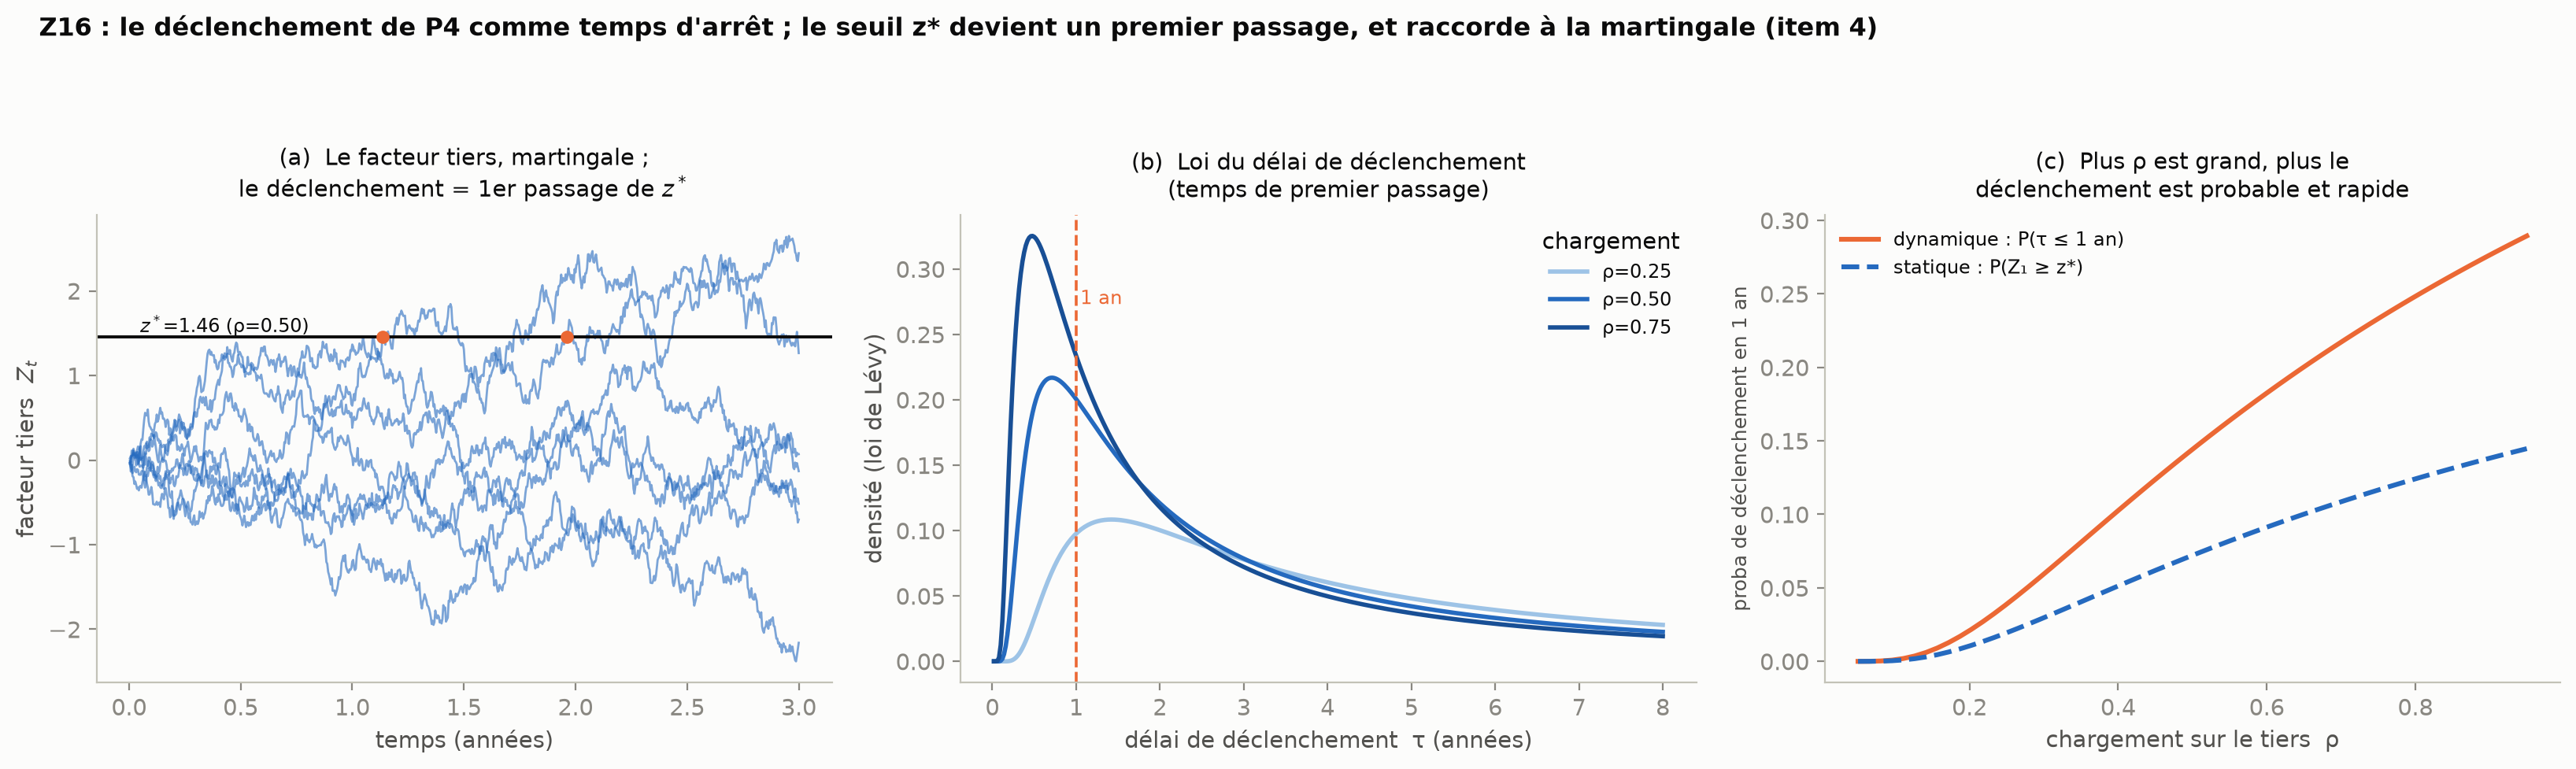
\includegraphics[width=\linewidth]{Z16_p4_temps_arret.png}\\[2pt]
{\scriptsize Si le facteur tiers est un \textbf{processus}, le seuil devient un \textbf{temps
d'arrêt} : le \og{}moment\fg{} de déclenchement a un sens littéral, et rejoint le cadre
martingale de la troisième piste.}
\end{column}
\end{columns}
\end{frame}

% =====================================================================
\begin{frame}{Points bloquants et pour la prochaine fois}
\small
\textbf{Ce qui dépend d'autres que moi}
\begin{itemize}\itemsep1pt
\item Les \textbf{deux relectures} demandées : elles lèveraient la dernière réserve sur la
      direction, et le délai de retour est le seul facteur hors de mon contrôle.
\item Le \textbf{registre d'externalisation} : le squelette d'ingestion est prêt, il n'attend
      que la donnée.
\item Le \textbf{choix de posture} sur le capital : point prédictif ou borne prudente ? À
      trancher avec Caroline, les deux sont chiffrés.
\end{itemize}
\textbf{Livré depuis le 24/07}
\begin{itemize}\itemsep1pt
\item Les quatre pistes, puis le chapitre sur l'\textbf{identifiabilité réécrit} : d'un verdict
      unique à une frontière en trois niveaux.
\item Le mémoire \textbf{restructuré en cinq parties} selon les attendus de l'Institut, et
      \textbf{treize fiches} autonomes.
\end{itemize}
\vfill
\begin{block}{}
Ligne de conduite inchangée : ne jamais présenter comme mesuré ce qui est posé, ni comme
calibré ce qui n'est que corroboré.
\end{block}
\end{frame}

\end{document}
